Dựa trên ma trận hiệp phương sai lịch sử, bài toán tối ưu hóa Mean-Variance (Markowitz) được giải quyết bằng thuật toán SLSQP nhằm tìm ra danh mục tiếp điểm có tỷ số Sharpe cực đại.

\begin{figure}[H]
    \centering
    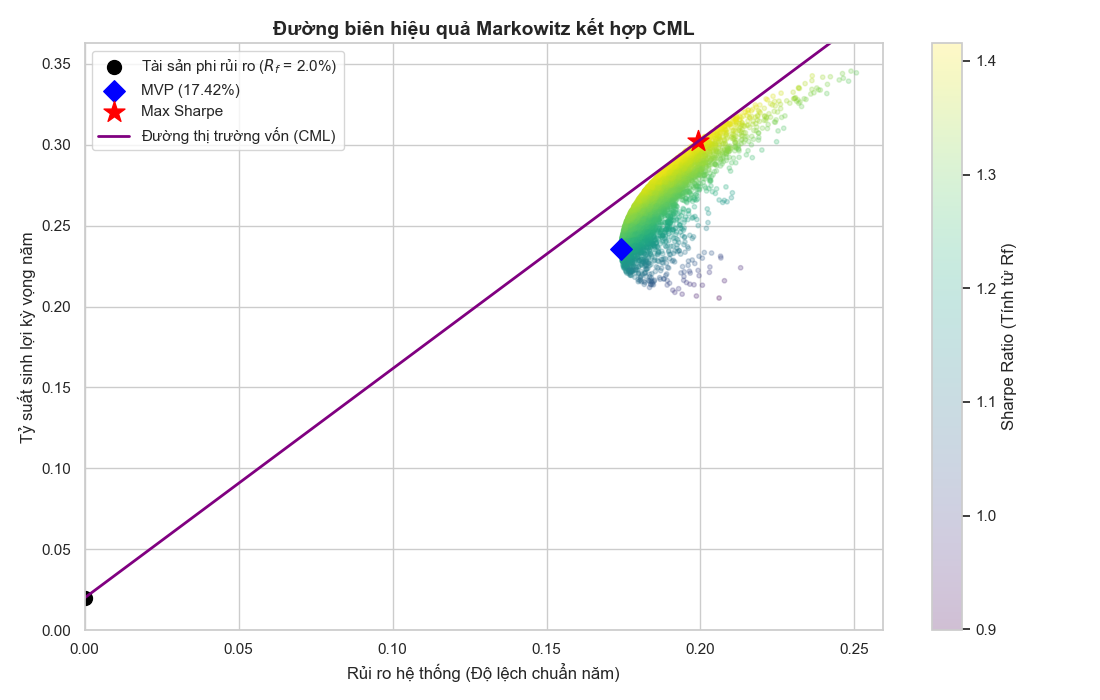
\includegraphics[width=0.85\textwidth]{efficient_frontier_with_cml.png}
    \caption{Đường biên hiệu quả Markowitz và Đường thị trường vốn (CML)}
    \label{fig:markowitz}
\begin{flushleft}
\textbf{Nhận xét Hình \ref{fig:markowitz}:} 
Đồ thị biểu diễn hàng ngàn kịch bản danh mục mô phỏng (các điểm màu) tạo thành đường biên hiệu quả. Điểm ngôi sao màu đỏ đại diện cho danh mục tối ưu Max Sharpe, nơi đường thị trường vốn (CML) tiếp xúc với đường biên. Tại điểm này, thuật toán đề xuất mức phân bổ vốn tối ưu là: AAPL (18.45\%), MSFT (40.96\%), AMZN (4.06\%), và GOOGL (35.99\%). Danh mục này mang lại mức lợi nhuận kỳ vọng 29.66\%/năm với rủi ro biến động 19.55\%/năm và tỷ lệ Sharpe tối ưu lớn nhất là 1.5172. Bộ tỷ trọng này sẽ được cố định để làm cơ sở cho mô phỏng Copula ở các bước sau.
\end{flushleft}
\end{figure}
